\documentclass[class=report, crop=false]{standalone}
\usepackage[subpreambles=true]{standalone}
\usepackage{import}

\begin{document}
Ground station's task is communicating with the CanSat and analyzing its sensor readings. \\
To achieve that we are going to to use:
\begin{itemize}
\item a long-range radio transceiver 
\item a Yagi antenna 
\item a ground station computer
\item a data processing unit.
\item additional equipment for the SatTrack system 
\end{itemize}
\subsection*{Communication module}
The communication module shall consist of a Lo-Ra transceiver and a Yagi antenna. \\
This component will be responsible for two-way communication with the satellite. \\
For the transmitter-receiver, we will use a mainboard from the CanSat kit (SX-1278 to be exact). \\
For the antenna, we are using a 433MHz Yagi-Uda antenna. \\
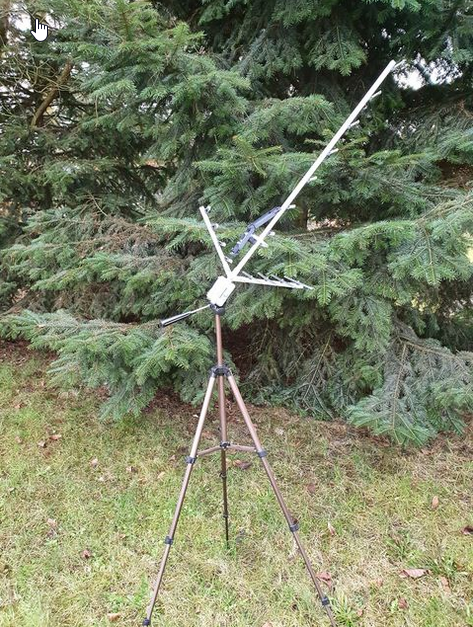
\includegraphics[width=\columnwidth]{ext/radio.png}
\captionof{figure}{Antenna we built and are going to use}
\newpage
\subsection*{Ground station computer}
The ground station computer will act as a bridge between the data processing unit and the communication module. \\
Its job is to receive data from the CanSat via the communication module and transfer it to the data processing unit. \\
Additionally, the computer will control the SatTrack system. \\
\subsection*{The SatTrack tracker}
SatTrack tracker is a system that adjusts the angle of the ground station antenna. \\
The mechanism consists of a rotator that will adjust the angle of the antenna accordingly. \\
This device is controlled by the ground station computer. \\
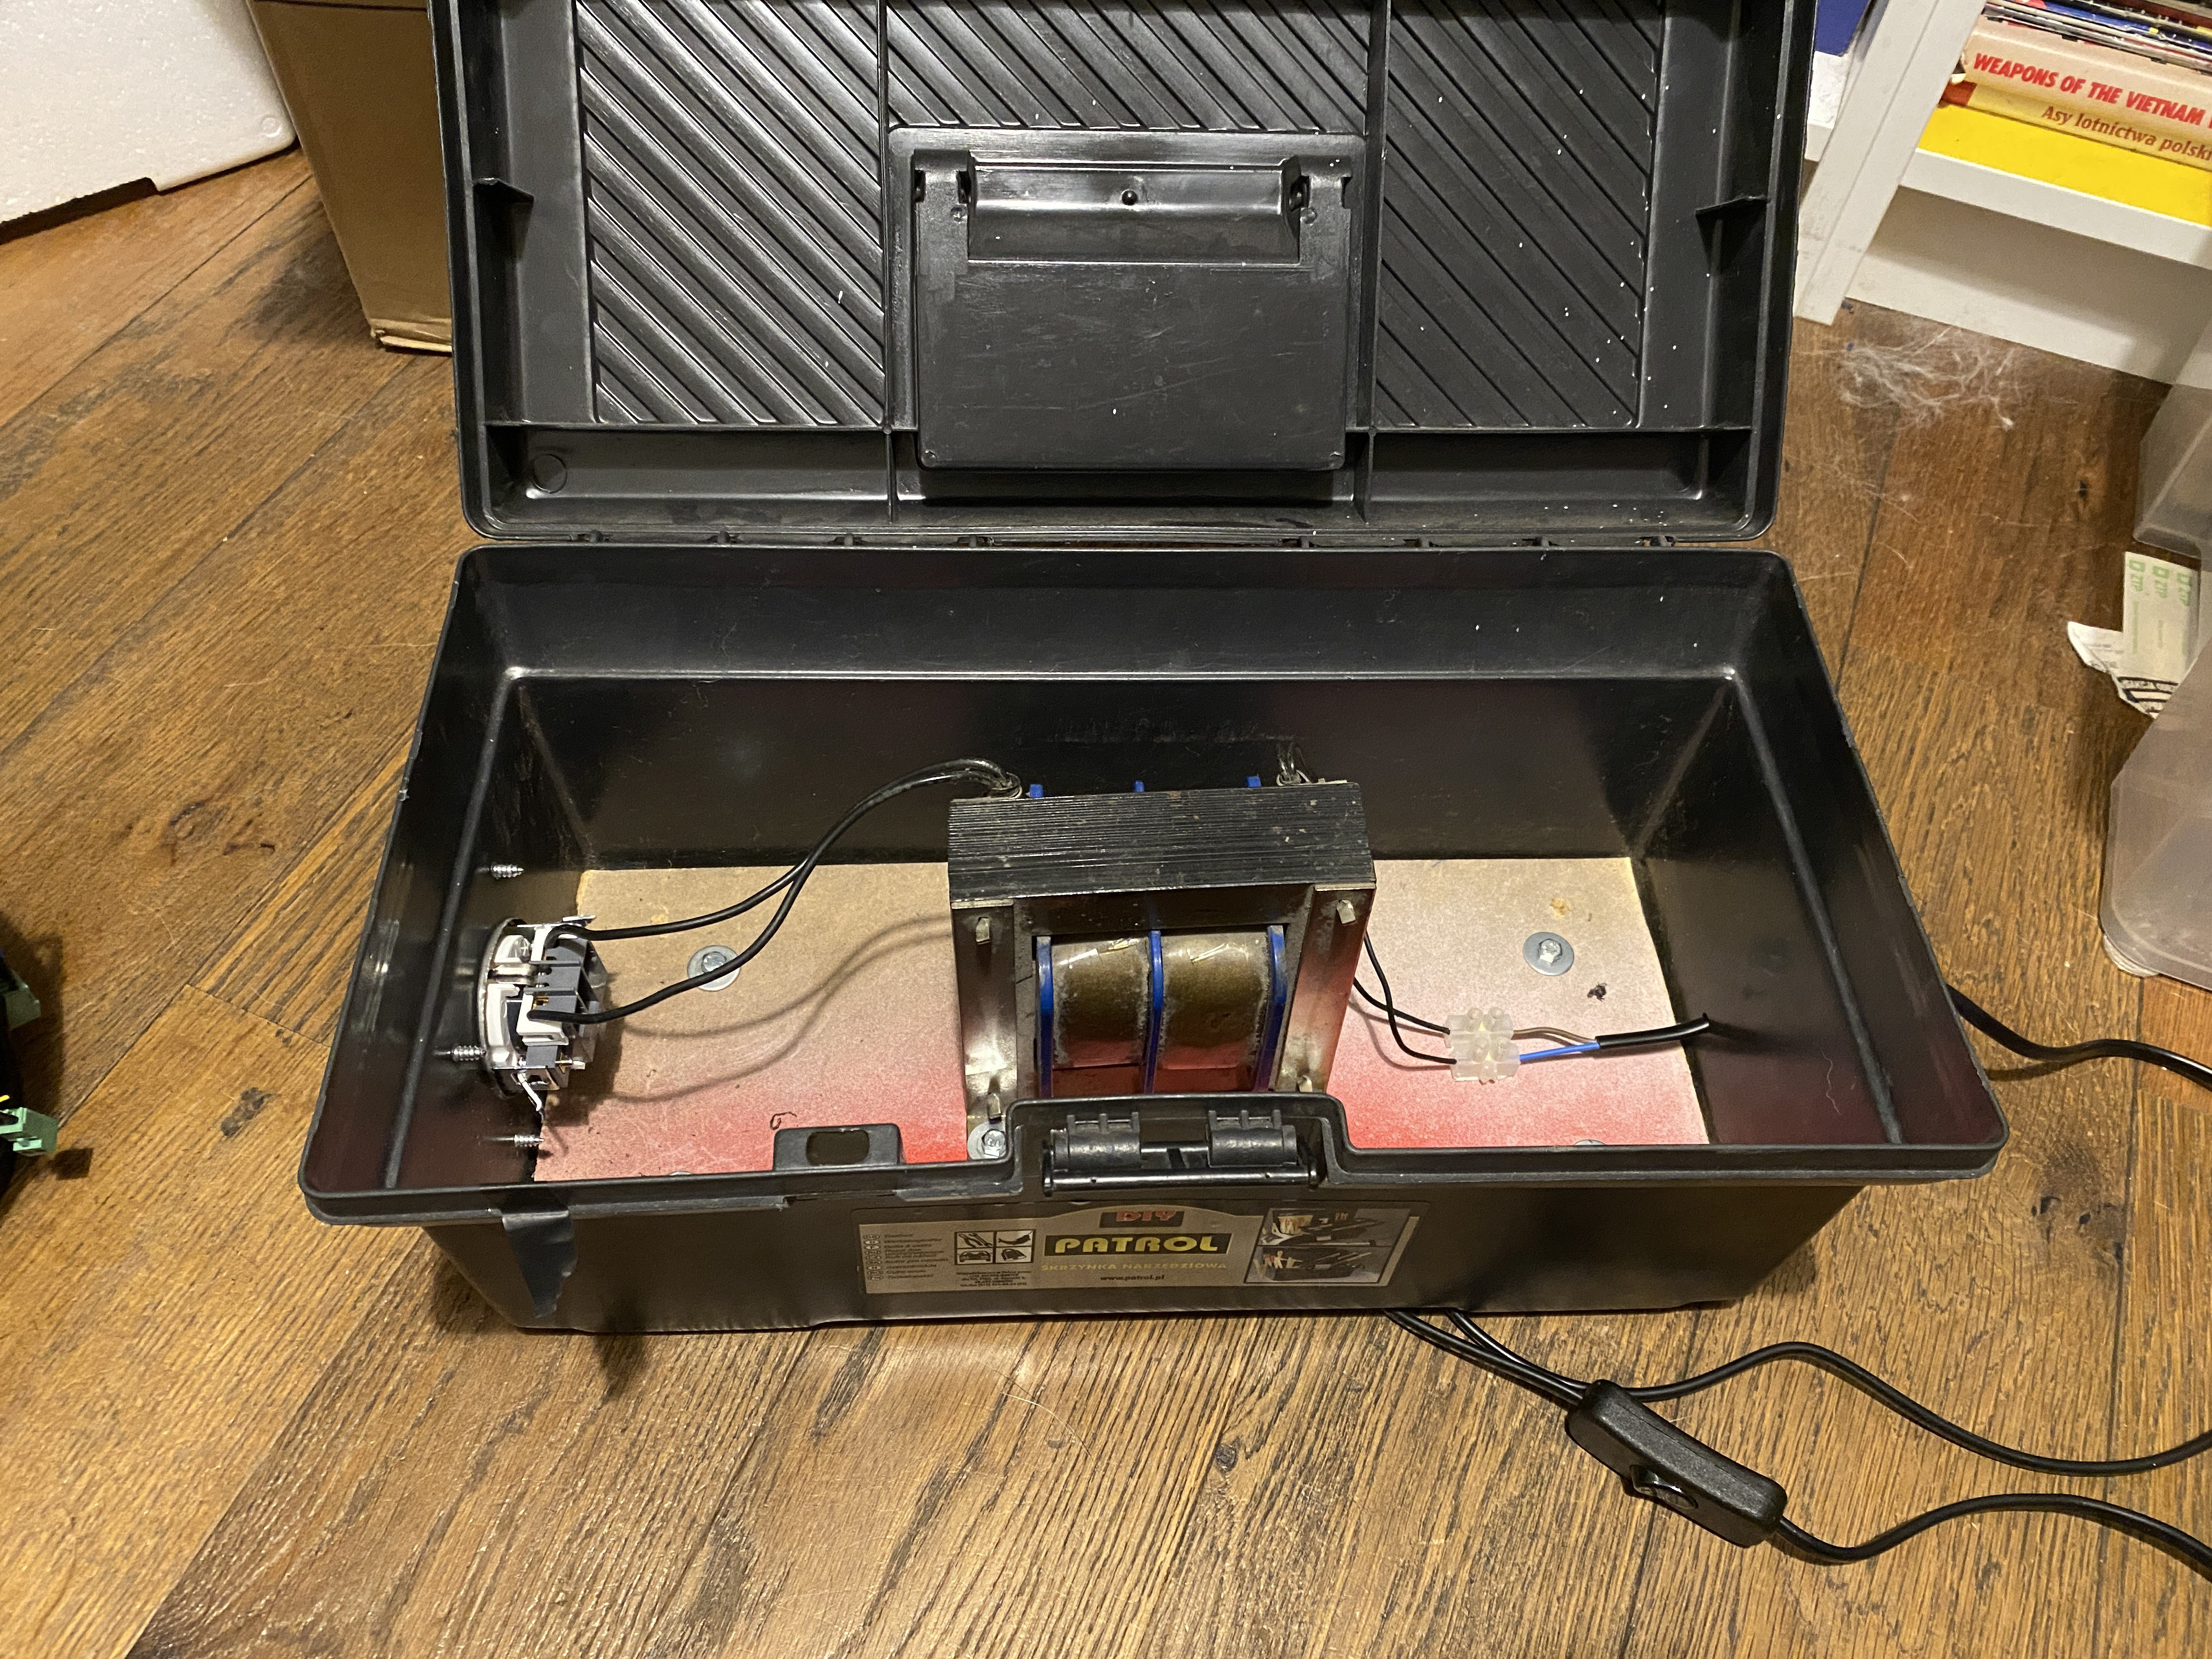
\includegraphics[width=\columnwidth]{ext/sattrackpower.png}
\captionof{figure}{Power transformer for the motors and equipment}
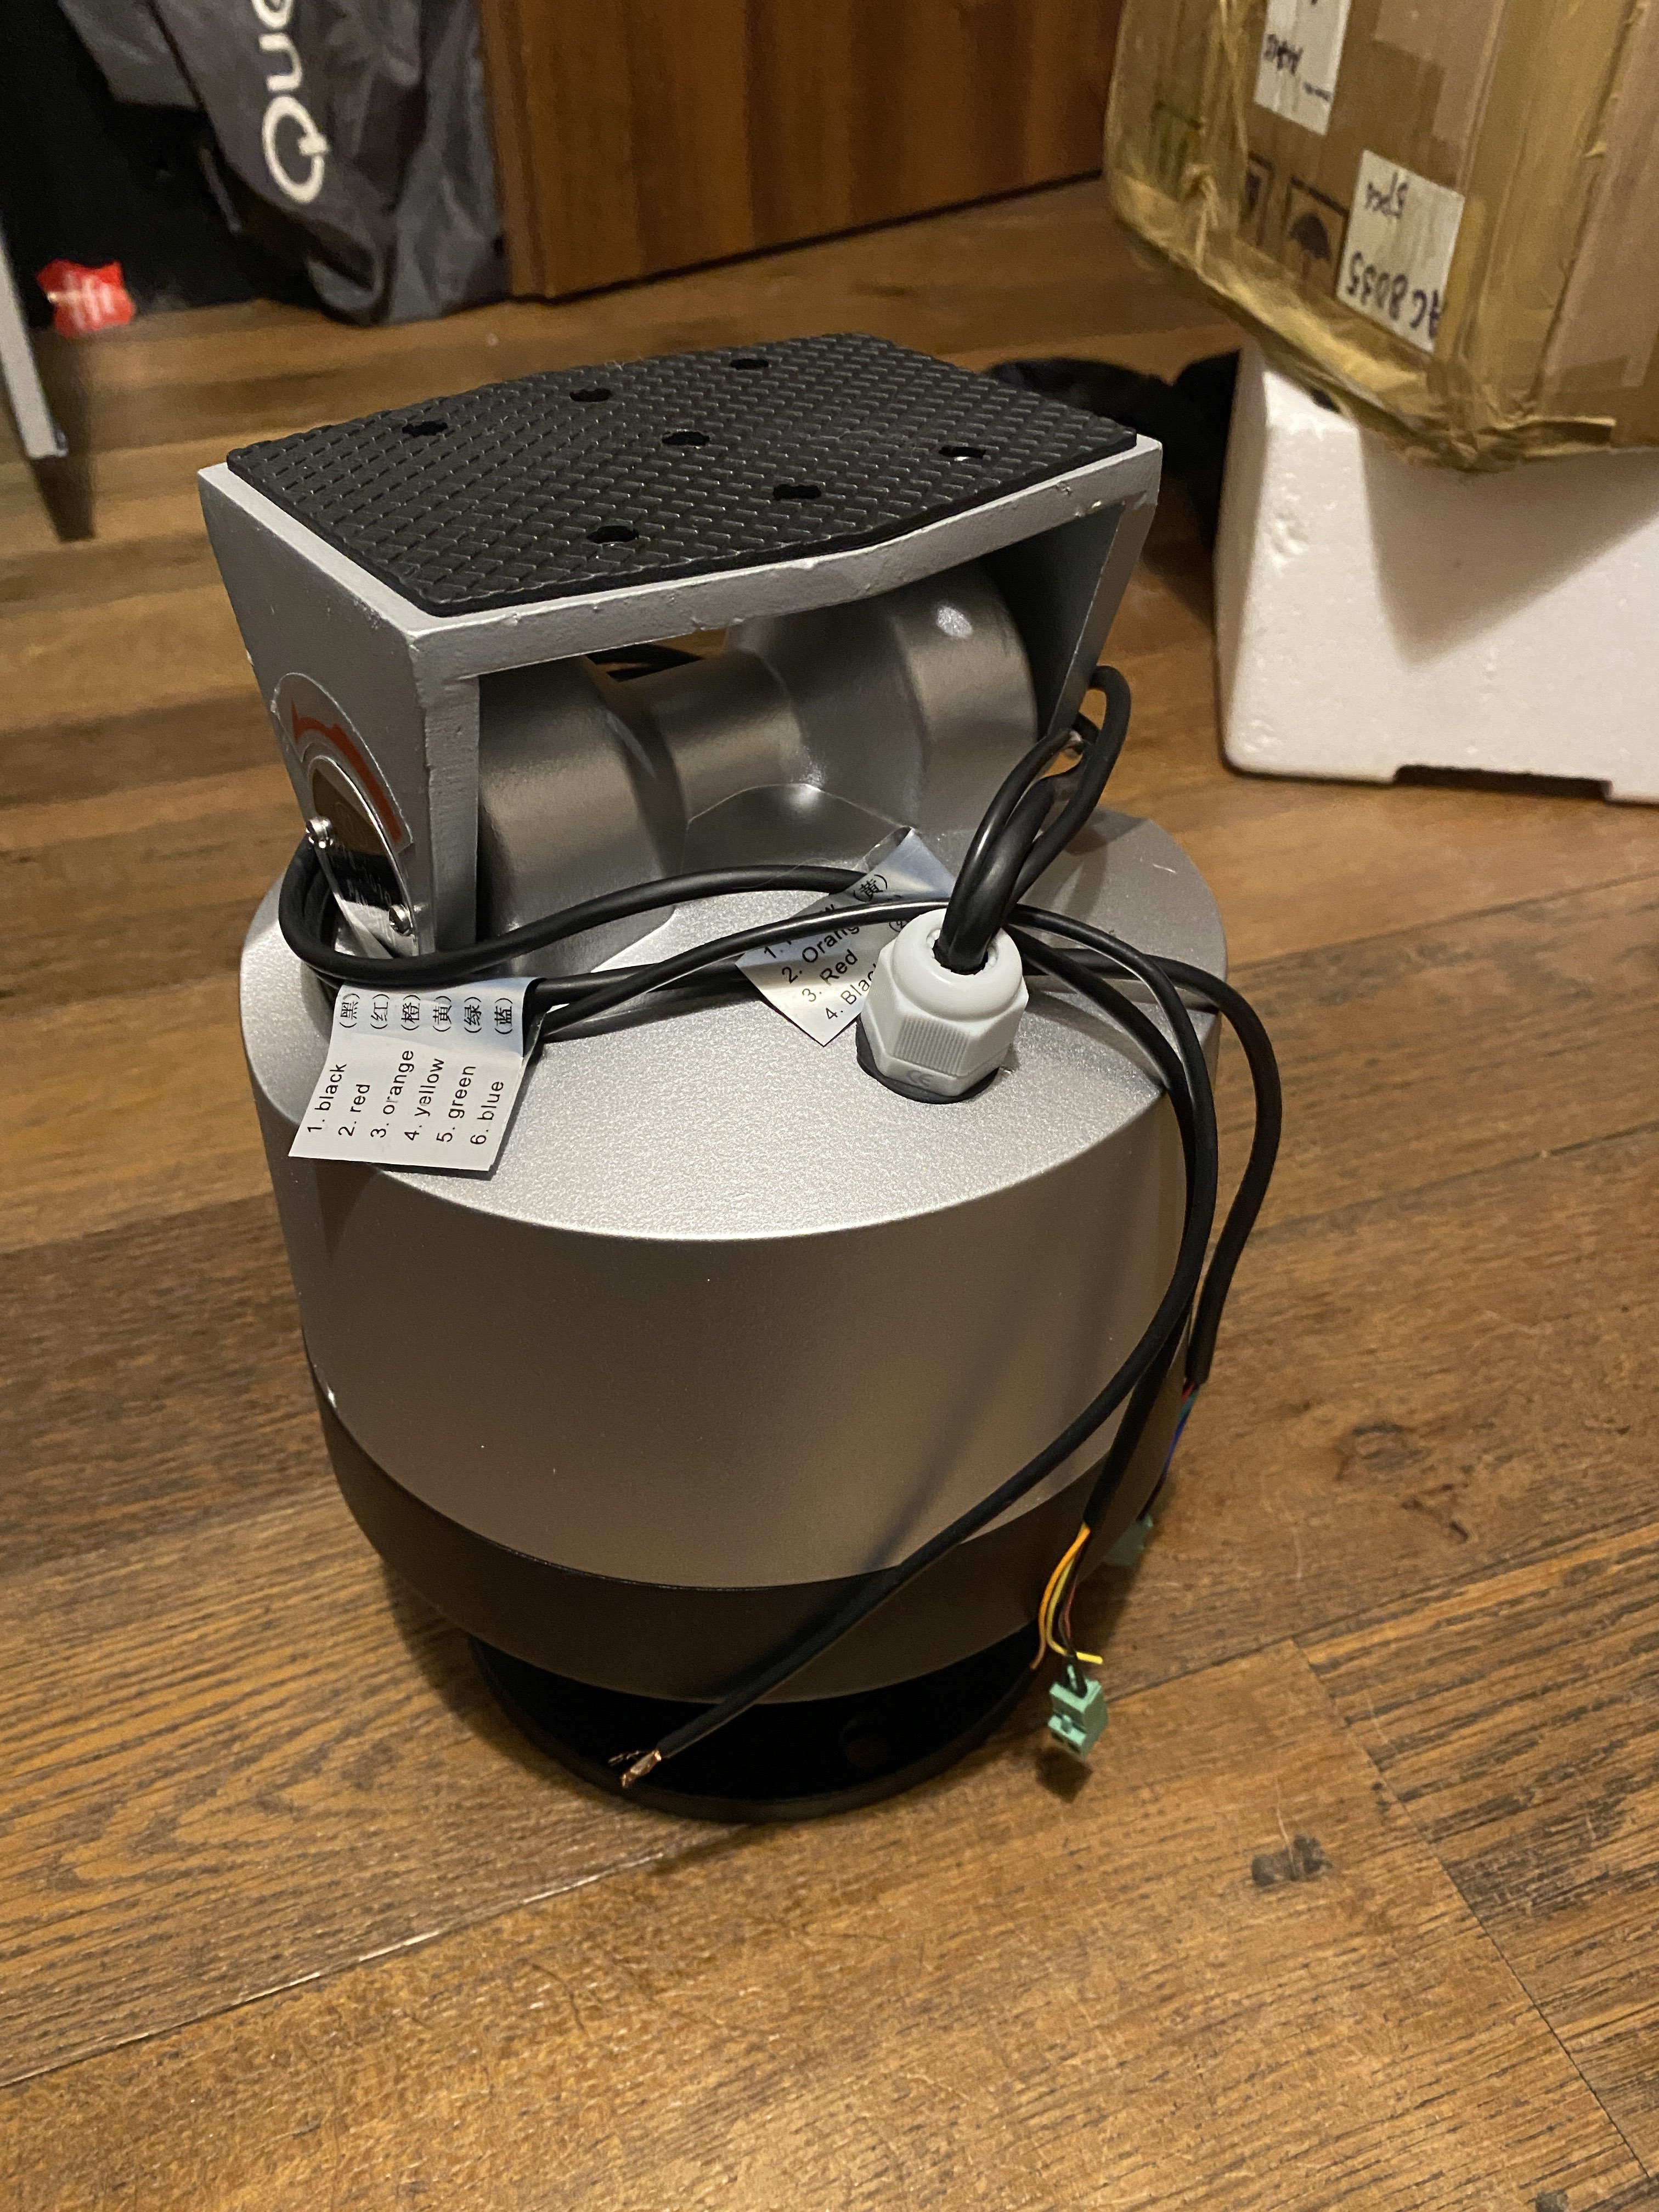
\includegraphics[width=\columnwidth]{ext/sattrackrotate.png}
\captionof{figure}{The rotating part of SatTrack}
\subsection*{Data processing unit}
The data processing unit will be a laptop of one of the members. \\
Its job will be to receive and analyze data from the ground station computer. \\
This includes, but is not limited to saving the data to a hard drive and graphing it in real time.
\end{document}
